% Author: Prof. Dr. Matthias Jung, DL9MJ
% Year: 2023
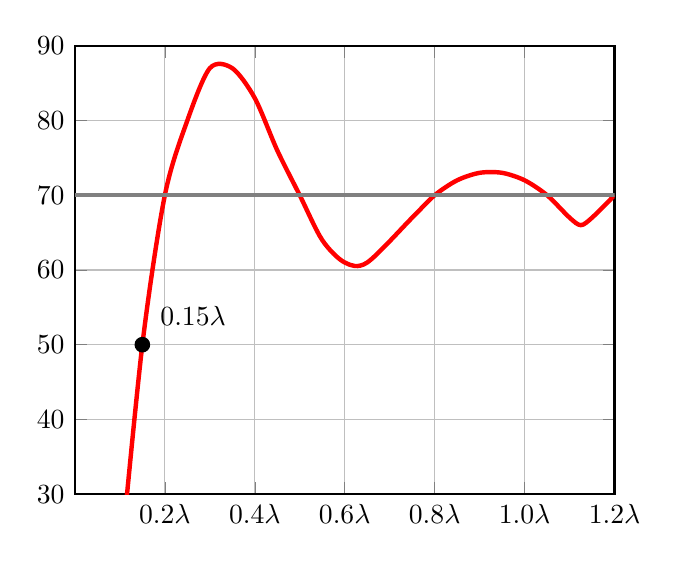
\begin{tikzpicture}
    \pgfplotsset{samples=200}
    \begin{axis}[
        %ticks=none,
        xmin =  0,
        ymin = 30,
        xmax = 1.2,
        ymax = 90,
        %domain = 0:6,
        grid=both,
        ytick = {30,40,50,60,70,80,90},
        xtick = {0,0.2,0.4,0.6,0.8,1.0,1.2},
        xticklabels = {$~$,0.2$\lambda$,0.4$\lambda$,0.6$\lambda$,0.8$\lambda$,1.0$\lambda$,1.2$\lambda$},
        thick,
        smooth,
        no markers]
        \addplot[smooth, ultra thick, color=red] coordinates {
            (0.10,20)
            (0.15,50)
            (0.20,70)
            (0.25,80)
            (0.30,87)
            (0.35,87)
            (0.40,83)
            (0.45,76)
            (0.50,70)
            (0.55,64)
            (0.60,61)
            (0.65,61)
            %(0.70,65)
            (0.75,67)
            (0.80,70)
            (0.85,72)
            (0.90,73)
            (0.95,73)
            (1.00,72)
            (1.05,70)
            (1.10,67)
            (1.125,66)
            (1.15,67)
            (1.20,70)
	    };
        \addplot[smooth, ultra thick, color=gray] coordinates {
            (0.00,70)
            (0.10,70)
            (0.15,70)
            (0.20,70)
            (0.25,70)
            (0.30,70)
            (0.35,70)
            (0.40,70)
            (0.45,70)
            (0.50,70)
            (0.55,70)
            (0.60,70)
            (0.65,70)
            (0.75,70)
            (0.80,70)
            (0.85,70)
            (0.90,70)
            (0.95,70)
            (1.00,70)
            (1.05,70)
            (1.10,70)
            (1.15,70)
            (1.20,70)
	    };
        \node[label={~~~~~~~~~~~0.15$\lambda$},circle,fill,inner sep=2pt] at (axis cs:0.15,50) {};
    \end{axis}
\end{tikzpicture}